% ====================================================================
% Appendices
% ====================================================================
% After \appendix in thesis.tex, each \section here renders as
% Appendix A, B, C, ...

% ====================================================================
\chapter{Reproducibility Protocol, Manifest Hash Chain, and Verification Recipe}\label{app:repro}
% ====================================================================

This appendix documents the audit-first reproducibility protocol that underpins every numerical claim in this dissertation, following a model-card-style template inspired by the documentation discipline introduced for machine-learning artefacts \cite{Mitchell2019}. The protocol is implemented as a SHA-256 hash chain pinning every figure, table, and benchmark number to its inputs and the producing Git commit, and as a smoke-reproducibility harness that verifies the chain end-to-end on a fresh checkout in approximately five seconds.

\section{Per-Stage Manifest Pattern}\label{app:manifest_pattern}
Every development stage of the framework emits one or more \texttt{manifest.json} files under \texttt{docs/results/<phase>/} that record (a) the SHA-256 hash of every input artefact (data splits, trained models, scaler, episode roll-outs, upstream stage manifests), (b) the producing Git commit (\texttt{git\_sha}), and (c) the producing-script invocation (\texttt{produced\_by}). Each manifest also records the SHA-256 hash of every output artefact (figure, summary JSON, scoreboard) so that downstream stages can pin the upstream output by hash, not by filename alone. The per-stage artefact inventory is summarised in Table~\ref{tab:manifest_inventory}.

\begin{table}[!htbp]
\centering
\caption{Per-stage reproducibility-artefact inventory under \texttt{docs/results/}. \texttt{F<k>} entries are figures or tables, \texttt{G<n>\_scoreboard.json} are gate-evaluation scoreboards. Run-time roll-out JSONLs (under \texttt{runs/<phase>/}) are gitignored but their SHA-256 hashes are pinned by the stage manifest.}
\label{tab:manifest_inventory}
\begin{tabular}{l l l}
\hline
Stage & Path & Key artefacts \\
\hline
1 (Dataset prep.) & \texttt{01\_dataset/} & \texttt{F0\_class\_distribution.png}, \texttt{F0\_stage\_distribution.png}, \texttt{F0\_summary.json}, \texttt{manifest.json} \\
2 (Markov attacker) & --- & Closed-form $5\times5$ transition matrix (\texttt{MarkovAttacker}); no trained artefacts (requires no training) \\
3 (Env. design) & \texttt{03\_env/} & \texttt{PLAN.md}, \texttt{RESULTS.md} (no figures; environment is infrastructure) \\
4 (Stage detector) & \texttt{04\_detector/} & \texttt{F11\_per\_stage\_recall.png}, \texttt{F11\_summary.json}, \texttt{G4\_scoreboard.json}, \texttt{manifest.json}, \texttt{RESULTS.md} \\
5 (Blue-team DRL) & \texttt{05\_blue\_team/} & \texttt{F3/F4\_*.png}, \texttt{F3/F4\_summary.json}, \texttt{F3/F4\_manifest.json}, \texttt{T1\_hparams.\{json,md\}}, \texttt{G5\_scoreboard.json}, \texttt{RESULTS.md} \\
6 (Benchmark) & \texttt{06\_benchmark/} & \texttt{F5/F6/F7/F8\_*.png}, per-figure \texttt{summary.json} + \texttt{manifest.json} + \texttt{caption.md}, \texttt{G6\_scoreboard.json}, \texttt{RESULTS.md} \\
7 (Ablation/OOD) & \texttt{07\_ablation/} & \texttt{F9/F10/F12/F15\_*.png}, per-figure \texttt{summary.json} + \texttt{manifest.json} + \texttt{caption.md}, \texttt{G7\_scoreboard.json}, \texttt{RESULTS.md} \\
\hline
\end{tabular}
\end{table}

\section{Gate Scoreboards}\label{app:scoreboards}
Four \texttt{G<n>\_scoreboard.json} files (one per gated stage) record the threshold-vs.-observed value for every exit gate, the verdict bucketed into \textsc{pass} / \textsc{pass-with-finding} / \textsc{pass-without-stretch} / \textsc{fail-with-finding} / \textsc{fail} / \textsc{skip}, and a finding-id cross-reference where the verdict is contingent on a pre-registered finding-activation rule. Schema version 2.0 (Step-8 unification) is used uniformly across G4/G5/G6/G7. The verdict tally at the head of the dissertation's evaluation chain (commit \texttt{26b8df2}, the post-Step-8 \texttt{main}) is summarised in Table~\ref{tab:scoreboard_summary}.

\begin{table}[!htbp]
\centering
\caption{Gate-scoreboard summary across the four gated development stages. Verdicts are reported per-gate; the dissertation's headline-finding gates (G6.2 audit-AF2 reframe, G5.4 reward-hacking, G7.2 reward-component sweep, G7.9 OOD finding-activation) are highlighted.}
\label{tab:scoreboard_summary}
\begin{tabular}{l c c c c l}
\hline
Stage & \textsc{pass} & \textsc{pass-w/-finding} & \textsc{pass-w/o-stretch} & \textsc{fail-w/-finding} & Headline-gate ID \\
\hline
Stage detector (\texttt{G4}) & 4 & 1 & --- & --- & G4.4 (OOD recall asymmetry, $\Delta = 0.998$) \\
Blue-team DRL (\texttt{G5}) & 6 & 1 & --- & --- & G5.4 (prevention-rate primary KPI; best-algo prevention $0.602$) \\
Benchmark (\texttt{G6}) & 4 & 1 & --- & 1 & G6.2 (audit-AF2 reframe, \OracleCapturePct\,\% of oracle ceiling) \\
Ablation/OOD (\texttt{G7}) & 7 & 1 & --- & 2 & G7.2 (F9 \texttt{impact\_is\_terminal}=False, D7.1.1) \\
\hline
\end{tabular}
\end{table}

\section{Smoke-Reproducibility Harness}\label{app:r1}
The harness \texttt{scripts/reproducibility\_smoke.py} is the canonical end-to-end verification recipe. It walks every committed \texttt{manifest.json} file under \texttt{docs/results/} and verifies, for every recorded input SHA-256, that the on-disk SHA-256 of that input \emph{right now} matches the recorded one. Output is bucketed into four categories:

\begin{description}
    \item[\textsc{ok}] The recorded input SHA matches the on-disk SHA. The expected case for every input.
    \item[\textsc{fail}] The recorded input SHA does \emph{not} match the on-disk SHA, and the divergence is not on the harness's pre-registered known-divergences list. This indicates that an input artefact has changed since the producing manifest was emitted, and the figure or scoreboard pinned by that manifest is no longer reproducible-by-hash from the inputs on disk. \textsc{fail} verdicts must be triaged.
    \item[\textsc{known-divergence}] The recorded SHA does not match on-disk \emph{and} the divergence is documented and audited. The harness ships with a \texttt{\_KNOWN\_DIVERGENCES} table that explicitly enumerates every such case with its finding-id and explanatory note. The pre-registered divergence in this dissertation is the dataset-preparation stage manifest's recorded splits-manifest SHA (\texttt{82aa1214\ldots}, the pre-leakage-fix manifest) versus the on-disk post-fix SHA; the splits manifest is gitignored machine-local data, regenerated per machine, and the input is absent (\textsc{skip}) on a fresh clone.
    \item[\textsc{skip}] An input declared by the manifest is gitignored and not on disk on this checkout. Typical case: large feature arrays (\texttt{features.npy}, \texttt{stages.npy}) and split index files that are derived from the raw CICIoT2023 dataset and therefore not committed.
\end{description}

The harness's verdict at the head of the dissertation's evaluation chain is \textbf{\textsc{pass}}: all SHA-256 checks pass, with 0 \textsc{fail} verdicts; the pre-registered 2 \textsc{known-divergence} entries (the pre- and post-leakage-fix splits manifests) and a small number of \textsc{skip} verdicts (gitignored raw-data artefacts) are the expected outcome on a fresh checkout. A non-zero \textsc{fail} count would block merge of any commit that introduces it.

\section{Verification Recipe (Fresh-Checkout Reproduction)}\label{app:recipe}
On a fresh checkout, the empirical record can be re-verified end-to-end without retraining any model:

\begin{verbatim}
git clone <repo-url> rl-iot-defense-system
cd rl-iot-defense-system
python -m venv .venv && source .venv/bin/activate
pip install -r requirements.txt
pytest -q                                        # expect: \NumTests{} passed
python -m scripts.reproducibility_smoke         # expect: VERDICT PASS
                                                 #         0 FAIL / 2 KNOWN-DIVERGENCE
\end{verbatim}

The dissertation PDF is compiled via a local container image (Podman, with Docker as a fallback; no host-side \LaTeX{} installation required):

\begin{verbatim}
# Compile tex/main.pdf (auto-builds the image if absent):
make thesis

# Alternatively, use the standalone script from the repo root
# (auto-detects and prefers Podman):
bash tex/build.sh
\end{verbatim}

A full re-train of every stage from scratch (preserving the audited reproducibility contract) is also supported via \texttt{make}:

\begin{verbatim}
make dataset                              # CICIoT2023 splits + F0a/F0b
                                          # (requires raw dataset on disk)
make detector                             # supervised stage detector + F11
make blue-team-sweep BLUE_TEAM_TIMESTEPS=250000   # ~108 min CPU
make benchmark                            # held-out benchmark + F5/F6/F7/F8
make ablation                             # ablations + F9/F10/F12/F15 (~7.5 h CPU)
make ablation-close                       # G7 scoreboard + RESULTS.md
\end{verbatim}

After a full re-train the per-stage \texttt{manifest.json} files are re-emitted with new input SHAs corresponding to the freshly trained checkpoints; the harness will then verify the new chain end-to-end.

\section{Hardware and Environment}\label{app:hardware}
All experiments reported in this dissertation were run on a single CPU core. No GPU is required for any development stage (the MLP stage detector and the three DRL agents all train within minutes-to-hours on commodity CPU; the $5\times5$ Markov attacker is closed-form and requires no training). Software environment: Python 3.10--3.11 (CI-verified), PyTorch (CPU build), scikit-learn, Stable~Baselines3, Gymnasium. Total wallclock for the full audited evaluation chain (development stages 1--7) is approximately 8.5~h on a single CPU core, dominated by the ablation sweeps; the held-out benchmark and the smoke-reproducibility harness together take less than 11~minutes.

% ====================================================================
\chapter{CICIoT2023 Label to Kill Chain Stage Mapping}\label{app:kc_mapping}
% ====================================================================

The 34 CICIoT2023 labels (33 attack classes plus \texttt{BenignTraffic}) are projected onto the five Kill Chain stages defined in Section~\ref{sec:kill_chain} via the closed mapping in Table~\ref{tab:kc_mapping}. The mapping is implemented in \texttt{src/utils/label\_mapper.py::AbstractStateLabelMapper}; an unknown label encountered at processing time raises an explicit \texttt{KeyError} so that any new attack class added to the dataset cannot silently leak into an existing stage. The full design rationale, including why the Lockheed Martin seven-step chain is coarsened to five stages here and why the $\textsc{benign} \to \textsc{recon} \to \textsc{access} \to \textsc{maneuver} \to \textsc{impact}$ ordering is monotone in attacker progress, is provided in \texttt{docs/kill-chain-mapping.md}.

\begin{table}[!htbp]
\centering
\caption{Per-class CICIoT2023 to Kill Chain stage mapping. Classes marked $^\star$ are reserved as held-out out-of-distribution attack classes (Section~\ref{ssec:splits}) and are never seen during training of either the supervised stage detector or the DRL agents.}
\label{tab:kc_mapping}
\begin{tabular}{l p{10cm}}
\hline
Stage & CICIoT2023 labels \\
\hline
\textsc{benign}  & \texttt{BenignTraffic} \\
\hline
\textsc{recon}   & \texttt{Recon-PortScan}, \texttt{Recon-OSScan}, \texttt{Recon-HostDiscovery}, \texttt{Recon-PingSweep}, \texttt{VulnerabilityScan}$^\star$ \\
\hline
\textsc{access}  & \texttt{BrowserHijacking}, \texttt{CommandInjection}, \texttt{SqlInjection}, \texttt{Backdoor\_Malware}, \texttt{Uploading\_Attack}, \texttt{XSS}$^\star$, \texttt{DictionaryBruteForce} \\
\hline
\textsc{maneuver} & \texttt{MITM-ArpSpoofing}, \texttt{DNS\_Spoofing}, \texttt{Mirai-greeth\_flood}, \texttt{Mirai-greip\_flood}, \texttt{Mirai-udpplain}$^\star$ \\
\hline
\textsc{impact}  & DoS variants (\texttt{DoS-TCP\_Flood}, \texttt{DoS-UDP\_Flood}, \texttt{DoS-SYN\_Flood}, \texttt{DoS-HTTP\_Flood}); DDoS variants (\texttt{DDoS-TCP\_Flood}, \texttt{DDoS-UDP\_Flood}, \texttt{DDoS-SYN\_Flood}, \texttt{DDoS-RSTFINFlood}, \texttt{DDoS-PSHACK\_Flood}, \texttt{DDoS-SynonymousIP\_Flood}, \texttt{DDoS-ICMP\_Flood}, \texttt{DDoS-ICMP\_Fragmentation}, \texttt{DDoS-UDP\_Fragmentation}, \texttt{DDoS-ACK\_Fragmentation}, \texttt{DDoS-SlowLoris}, \texttt{DDoS-HTTP\_Flood}$^\star$) \\
\hline
\end{tabular}
\end{table}

% ====================================================================
\chapter{Hyperparameters per Algorithm}\label{app:hparams}
% ====================================================================

The blue-team training hyperparameter table (T1) for DQN, PPO, and A2C is reproduced in Table~\ref{tab:hparams} from \texttt{docs/results/05\_blue\_team/T1\_hparams.json}, which is the canonical hash-pinned source. All values are Stable~Baselines3 defaults, frozen for the thesis at PLAN \S8 D5.4; the same values are used across the ten seeds (\texttt{seed} $\in \{0, 1, \ldots, 9\}$) and the 250{,}000 environment steps per run. Empty cells indicate hyperparameters that do not apply to the algorithm (e.g.\ off-policy DQN-only fields are blank for the on-policy PPO and A2C rows).

\begin{table}[!htbp]
\centering
\caption{Blue-team training per-algorithm hyperparameters. Values are frozen at PLAN \S8 D5.4 and used across all \NumSeeds{} seeds and 250{,}000 environment steps per run. N/A indicates the hyperparameter does not apply to the algorithm.}
\label{tab:hparams}
\small
\begin{tabular}{l r r r r r r r r}
\toprule
algo & lr & $n_{\text{steps}}$ & $\gamma$ & $\lambda_{\text{GAE}}$ & ent\_coef & vf\_coef & batch\_size & $n_{\text{epochs}}$ \\
\midrule
A2C & $7\!\cdot\!10^{-4}$ & 5    & 0.99 & 1.00 & 0.000 & 0.50 & N/A  & N/A  \\
DQN & $1\!\cdot\!10^{-3}$ & N/A  & 0.99 & N/A  & N/A   & N/A  & 32   & N/A  \\
PPO & $3\!\cdot\!10^{-4}$ & 2048 & 0.99 & 0.95 & 0.010 & 0.50 & 64   & 10   \\
\bottomrule
\end{tabular}
\end{table}
\par\smallskip\noindent{\small\textit{Note: N/A = hyperparameter not defined for that algorithm family. $n_{\text{steps}}$ applies only to on-policy methods (PPO/A2C); batch\_size and $n_{\text{epochs}}$ apply only to PPO; $\lambda_{\text{GAE}}$, ent\_coef, vf\_coef apply only to actor-critic methods. DQN off-policy fields listed below.}}

For DQN-specific off-policy hyperparameters (replay buffer, exploration schedule, target-network update interval), the values used were: \texttt{buffer\_size} $= 50{,}000$, \texttt{learning\_starts} $= 1000$, \texttt{tau} $= 1.0$, \texttt{target\_update\_interval} $= 1000$, \texttt{exploration\_fraction} $= 0.10$, \texttt{exploration\_initial\_eps} $= 1.0$, \texttt{exploration\_final\_eps} $= 0.05$, \texttt{max\_grad\_norm} $= 0.5$. The complete machine-readable record is at \texttt{docs/results/05\_blue\_team/T1\_hparams.json}.

The ablation and OOD-robustness evaluations re-use the PPO hyperparameters above unchanged --- only the environment (\texttt{impact\_is\_terminal}, \texttt{p\_defender\_deescalation}) and the reward coefficients (\texttt{defense\_success\_bonus}, \texttt{penalty\_missed\_impact}, \texttt{reward\_proportional}, \texttt{reward\_benign\_passive}, \texttt{penalty\_disproportionate}) are perturbed.

% ====================================================================
\chapter{Sensitivity Sweep Figures}\label{app:sensitivity}
% ====================================================================

This appendix collects the three hyperparameter sensitivity sweep figures referenced in Section~\ref{cap:methodology} (§3.5.4--3.5.6). All sweeps use DQN (single seed) or PPO ($\times$10 seeds) with all other parameters held at their environment-design defaults; mean test reward on \texttt{test\_balanced} is the primary metric. 95\,\% bootstrap confidence intervals are shown as shaded bands.

\section{Defender De-escalation Probability Sweep (F10)}\label{app:deesc_sweep}

Figure~\ref{fig:app_f10} reproduces the F10 environment-difficulty sweep from Section~\ref{sec:ablation_results}. The parameter $p_{\mathrm{down}}$ controls the probability that a proportionate (correct) defender action de-escalates the attacker one stage down the kill chain under the tug-of-war dynamics; lower $p_{\mathrm{down}}$ is a harsher environment. The sweep establishes that the headline operating point $p_{\mathrm{down}} = 0.90$ keeps the MDP challenging enough to yield useful training signal while both the learned and oracle policies respond monotonically to environment difficulty.

\begin{figure}[!htbp]
    \centering
    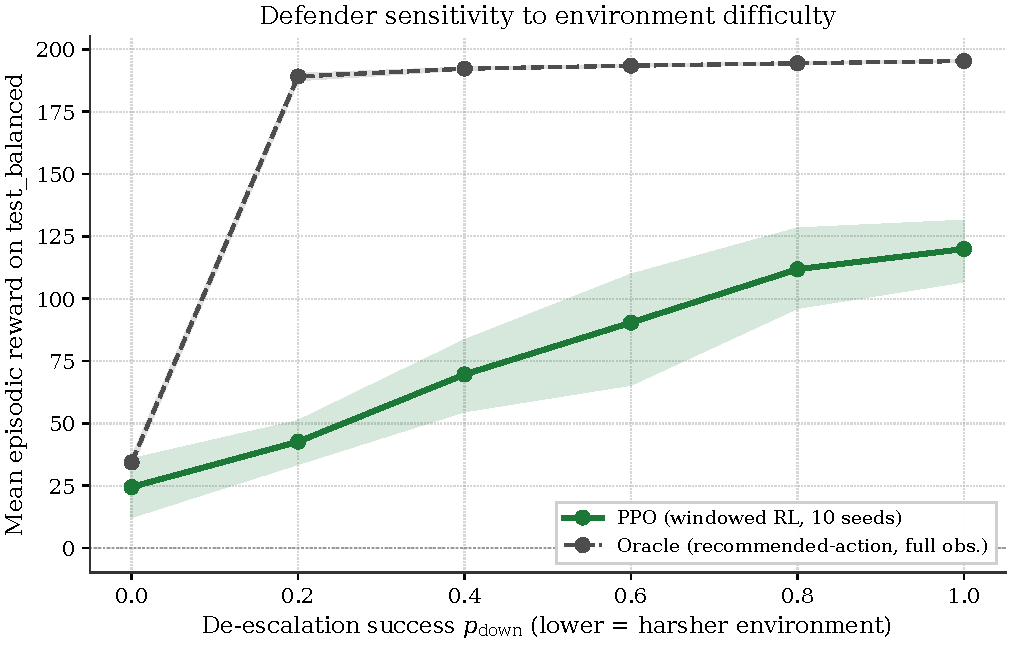
\includegraphics[width=0.85\textwidth]{figs/F10_aggressiveness.pdf}
    \caption{F10 environment-difficulty sweep: PPO mean test reward (10 seeds per point, shaded bands = 95\,\% bootstrap CIs) and oracle recommended-action rule reference across six values of the tug-of-war de-escalation success probability $p_{\mathrm{down}} \in \{0.0, 0.2, 0.4, 0.6, 0.8, 1.0\}$. PPO reward grows monotonically with $p_{\mathrm{down}}$; the headline operating point used throughout this dissertation is $p_{\mathrm{down}} = 0.90$.}
    \label{fig:app_f10}
\end{figure}

\section{Action-Cost Scale Sweep}\label{app:action_cost_sweep}

Figure~\ref{fig:app_fa_cost} shows the action-cost scale sensitivity sweep over $\alpha \in \{0.5, 1.0, 2.0\}$. All three settings produce overlapping 95\,\% bootstrap confidence intervals, confirming that the default $\alpha = 1.0$ is robust to $\pm 2\times$ perturbation.

\begin{figure}[!htbp]
    \centering
    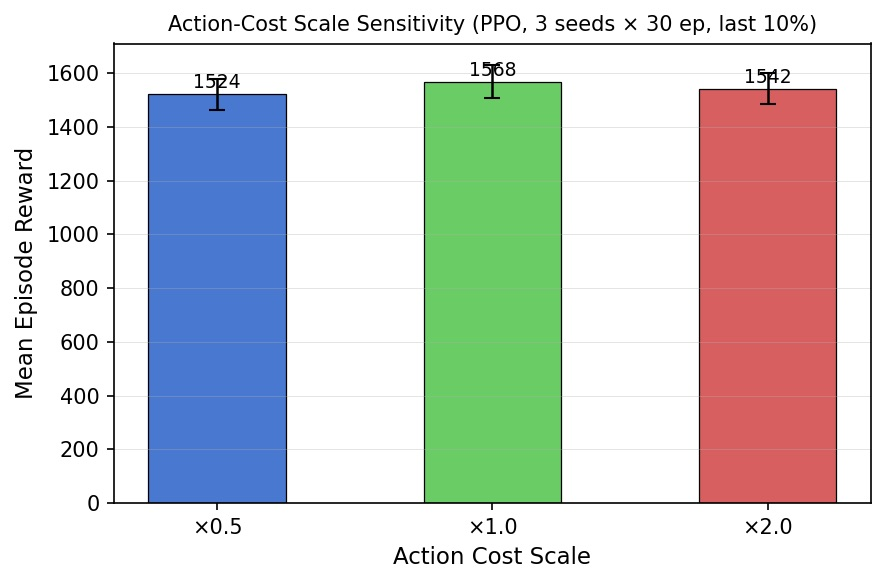
\includegraphics[width=0.75\textwidth]{figs/action_cost_sweep.pdf}
    \caption{Action-cost scale sensitivity sweep: mean test reward (DQN, seeds 0--2, 63 episodes per seed) at $\alpha \in \{0.5, 1.0, 2.0\}$. Error bars are 95\,\% bootstrap CIs. All CIs overlap; reward varies less than 3\,\% across the full range. Numeric values (reported on the pre-redesign reward scale, before the tug-of-war re-tuning; only the relative robustness conclusion carries over): $\alpha=0.5$: $+1524$ CI $[1462, 1579]$; $\alpha=1.0$: $+1568$ CI $[1506, 1628]$; $\alpha=2.0$: $+1542$ CI $[1484, 1600]$.}
    \label{fig:app_fa_cost}
\end{figure}

\section{History Window-Size Ablation}\label{app:window_ablation}

Figure~\ref{fig:app_fa_window} shows the window-size ablation over $w \in \{1, 3, 5, 10\}$. Window $w = 5$ achieves the highest mean reward; increasing to $w = 10$ does not improve reward while doubling the observation dimension from 290 to 580 features.

\begin{figure}[!htbp]
    \centering
    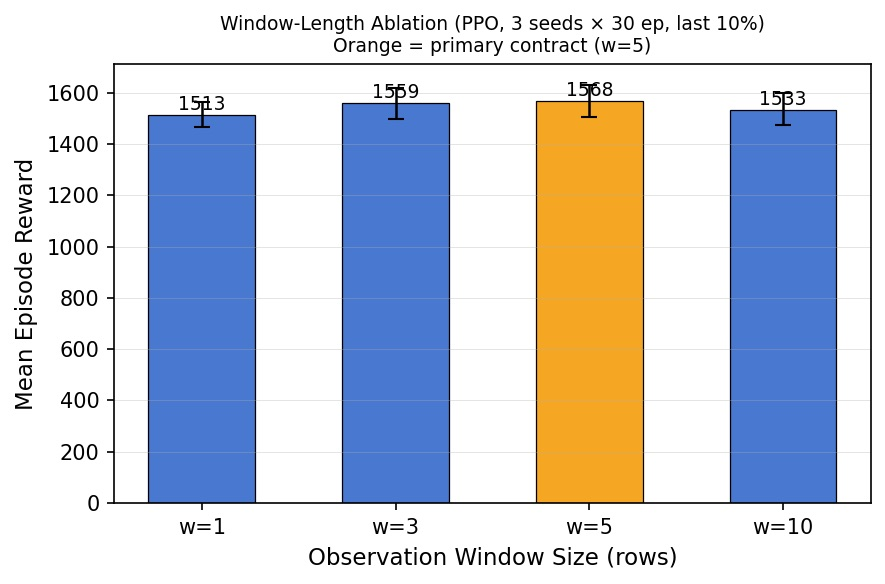
\includegraphics[width=0.75\textwidth]{figs/window_ablation.pdf}
    \caption{History window-size ablation: mean test reward (DQN, seed 0, 189 episodes) at $w \in \{1, 3, 5, 10\}$. Error bars are 95\,\% bootstrap CIs. Peak at $w = 5$ ($+1568$ CI $[1506, 1628]$; reported on the pre-redesign reward scale, only the relative ordering carries over); $w = 10$ is lower but CIs overlap ($+1533$ CI $[1472, 1599]$). Observation dimension is listed in parentheses.}
    \label{fig:app_fa_window}
\end{figure}
